Über die URL \url{https://nc.electribez.de/index.php/login} kommt ihr zur Verwaltungskonsole auf unserem Raspi-Nextcloud Server. Dort könnt ihr euer Password ändern, welches ihr vom Admin zugewiesen bekommen habt.\\

\begin{minipage}[t]{\textwidth}
  \centering
  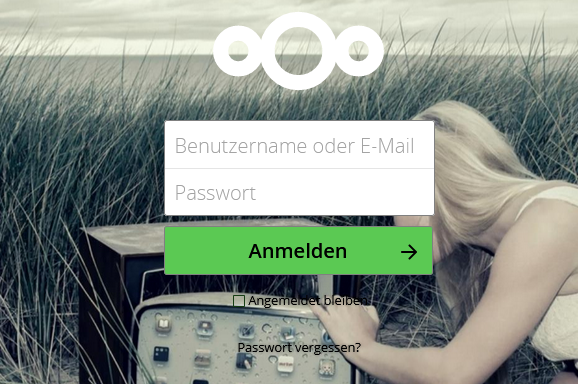
\includegraphics[height=5cm]{pictures/Nextcloudlogin.png}
  \captionof{figure}{Nextcloud Login}
  \label{img:Nextcloudlogin}
\end{minipage}


\subsection{Client Installieren}
Passende Clienten findet ihr auf \url{https://nextcloud.com/install/}\\
\ \\
Der Nexcloud Clienent stellt euch einen ständig Aktualisierte Kopie des Servers in C:\textbackslash Users\textbackslash Username\textbackslash Nextcloud zur Verfügung. Dort können wir gemeinsam an Inhalten arbeiten. Vorsicht, wenn 2 Leute an einen Thema arbeiten.\\
 
\begin{minipage}[t]{\textwidth}
  \centering
  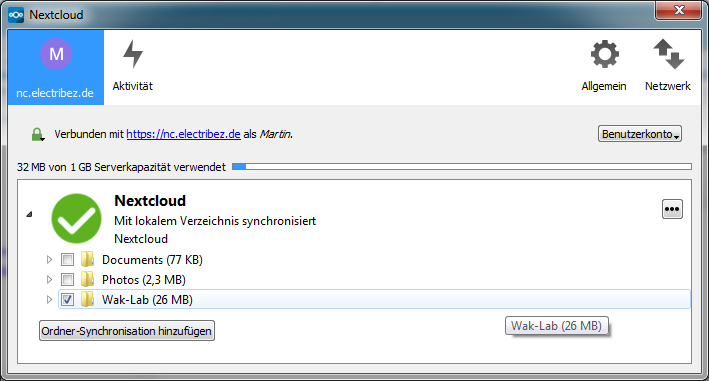
\includegraphics[height=5cm]{pictures/NextcloudWinClient.png}
  \captionof{figure}{Nextcloud Windows Client}
  \label{img:NextcloudWinClient}
\end{minipage}





